\documentclass[runningheads]{llncs}

\usepackage[T1]{fontenc}
\usepackage[utf8]{inputenc}
\usepackage{graphicx}
\usepackage{booktabs}
\usepackage{tabularx}
\usepackage{longtable}
\usepackage{amsmath,amssymb}
\usepackage{url}
\usepackage{todonotes}
\usepackage{xcolor}

\newcommand{\red}[1]{\textcolor{red}{#1}}
\newcommand{\eb}[1]{\todo[inline,caption="",color=teal!20]{{\bf EB} #1}}
\newcommand{\ebside}[1]{\todo[caption="",color=teal!10,size=\tiny]{{\normalsize{\bf EB}} #1}}

\graphicspath{{figures/}}

\begin{document}

\title{Smart City Analytics for Sustainable Tourism: an AI-Driven Multi-Source Framework for Flow  Forecasting in a Historic Borough}
\titlerunning{Smart City Analytics for Sustainable Tourism}

\author{Anonymous Author(s)}
\authorrunning{Anonymous Author(s)}
\institute{}

\maketitle

\begin{abstract}
Managing visitor flows is a key challenge for smart cities and smart tourism destinations, particularly in small historic towns where tourism pressure can affect urban sustainability and public-space management. While Artificial Intelligence (AI) techniques have been widely applied to mobility forecasting in large metropolitan areas, limited evidence is available for small destinations characterized by sparse sensing infrastructures and heterogeneous data ecosystems.
This paper presents an AI-driven multi-source forecasting framework for visitor-flow analytics in the historic borough of Dozza, Italy. The proposed framework integrates pedestrian camera counts,  mobile-network indicators, weather observations and event-related information into a unified  data platform supporting multi-horizon forecasting. The study evaluates multiple machine learning models for people forecasting in Dozza.

Results show that  tree-based ensemble models achieve substantial reductions in forecasting error compared with the  baseline. Conversely, demographic indicators derived from mobile-network data remain strongly driven by temporal inertia. The findings demonstrate the value of AI-enabled urban analytics for supporting data-driven decision making in small smart tourism destinations and provide a replicable framework for sustainable visitor management in historic urban environments.
%We evaluate three target families: pedestrian entrances and exits, mobile-network nationality indicators, and age-band presence indicators. 

%The experimental design uses chronological train/test splits, rolling top-k feature validation, leakage-aware feature selection, strong persistence baselines, generalized linear models, tree ensembles, gradient boosting models, a two-stage ridge model, ablation, permutation importance, and SHAP summaries. 



\keywords{Smart Cities \and Artificial Intelligence \and Smart Tourism \and Urban Analytics \and  Flow Forecasting \and Mobile Network Data}
\end{abstract}

\section{Introduction}
\label{sec:introduction}

Despite the growing adoption of Artificial Intelligence and urban analytics in Smart City ecosystems, most mobility and crowd-flow forecasting studies focus on large metropolitan areas characterized by dense sensing infrastructures, extensive transportation networks, and abundant historical observations. Comparatively little attention has been devoted to small historic towns and tourism-oriented destinations, where data availability is often fragmented across heterogeneous sources and where visitor management plays a critical role in urban sustainability.
This gap is particularly relevant for smart tourism destinations, where local authorities increasingly seek AI-enabled decision-support tools capable of anticipating visitor peaks, improving public-space management, optimizing local services, supporting sustainable mobility policies and preserving cultural heritage. In these contexts, forecasting is not an end in itself but a key component of data-driven urban governance. Existing studies rarely investigate whether the integration of heterogeneous urban data sources—including pedestrian sensors, telecommunications data, weather observations and event information—can be effectively integrated into a unified analytics framework supporting operational decision making in small historic destinations.

To address this gap, this paper proposes and evaluates an AI-driven multi-source forecasting framework for smart tourism analytics in the historic borough of Dozza, Italy, with 6,569 inhabitants in 2024. Rather than focusing exclusively on predictive performance, the framework aims to demonstrate how heterogeneous urban data streams can be transformed into actionable intelligence for local administrations and destination managers. The main contributions are:
\begin{enumerate}
    \item The design of a reproducible AI-enabled urban analytics framework integrating pedestrian sensing, mobile-network indicators, weather observations, and event-related information into a unified decision-support environment.
    \item A comprehensive multi-horizon evaluation, at 1, 3, 6, 12, and 24 hours ahead, of machine learning models against forecasting baselines.
    \item An empirical assessment of how heterogeneous urban data sources contribute to forecasting different mobility-related target families, including pedestrian flows (entrances and exits), nationality indicators (Italian and foreign presences) and demographic aggregates (age-based visitor distributions).
    \item An interpretable AI analysis combining feature selection, ablation studies, permutation importance, and SHAP explanations to improve transparency, explainability, and trustworthiness in Smart City decision-support applications.
\end{enumerate}
 
The  objective is not only to improve forecasting accuracy but also to assess how Artificial Intelligence can support sustainable tourism governance in small historic destinations. More specifically, the study evaluates whether integrating heterogeneous urban data sources generates measurable benefits beyond those obtainable through simple temporal persistence.
This distinction is important because high predictive accuracy in mobility data may simply reflect temporal inertia rather than the effective exploitation of contextual information. Understanding when external data sources contribute meaningful predictive value is therefore essential for designing robust and operationally useful Smart City analytics systems.



The remainder of the paper is organized as follows. Section~\ref{sec:related}
summarizes related work on Smart City analytics, tourism forecasting, and mobility prediction.
Section~\ref{sec:methodologies} describes the dataset, preprocessing pipeline, targets,
models, feature selection strategy and evaluation metrics. Section~\ref{sec:results} reports the
experimental results and interpretability analyses. Section~\ref{sec:conclusions}
concludes with implications and limitations.

\section{Related Work}
\label{sec:related}
Recent advances in Artificial Intelligence have significantly expanded the role of urban analytics in Smart City ecosystems. However, most existing studies focus on metropolitan environments, while comparatively limited attention has been devoted to small historic destinations.

% Pedoni
Pedestrian and crowd-flow forecasting are commonly framed as spatio-temporal
prediction problems in which recent flow history is combined with calendar,
weather, and spatial information. Citywide crowd-flow models often assume dense
grids, graphs, or transport networks. ST-ResNet, for example, introduced a
deep residual architecture for citywide crowd-flow prediction on spatial grids
\cite{Zhang2017STResNet}, while graph-based recurrent models such as DCRNN
represent flows over transportation networks \cite{Li2018DCRNN}. Pedestrian
volume forecasting has also been studied at high spatio-temporal granularity
using enhanced learning models \cite{Jiang2022PedestrianGranularity}.

% Turism forecasting
Tourism forecasting has long combined time-series models, econometric variables,
and increasingly diverse digital traces. Reviews emphasize that forecasting
performance is context-dependent and that no single model class dominates all
tourism-demand problems \cite{Song2019TourismDemandReview}. Recent work has
explored deep learning (DL) \cite{Law2019TourismDemandDeep} and multi-source big data
for demand forecasting \cite{Li2020TourismBigData}.

The Dozza setting differs from these large-scale urban setups. The available
pedestrian data is not a dense sensor graph but a small set of access-point
cameras. This makes a tabular approach with lagged histories, calendar variables,
weather covariates, and mobile-network aggregates a defensible baseline before
moving toward graph or deep sequence architectures. %It also makes baseline comparison especially important: at a one-hour horizon, recent local counts can already explain a substantial fraction of the next value.

Events can strongly affect local visitor dynamics. Mobile-phone data have been
used for tourism event analytics \cite{Leng2021TourismEventAnalytics} and
event-aware architectures have been proposed for mobility nowcasting
\cite{Wang2022EASTNet}. Our case study uses a lighter tabular alternative:
event records are transformed into hourly intensity, distance, city, category,
lag, and rolling features. \red{They are evaluated under the same chronological
forecast-origin protocol as the other covariates: for each horizon, model inputs
are built only from information that would be available at the prediction time,
while future target values and same-hour target-family variables are excluded.}
This is intentionally more modest
than a dedicated event-aware neural architecture, but it is appropriate for a
small local dataset and makes ablation against non-event feature groups direct.

Mobile and passive mobility data is particularly relevant when official counts
are sparse or delayed. Passive mobile data have been used to study seasonal
tourism mobilities \cite{Zaragozi2021PassiveMobileTourism}, and mobility-derived
variables can improve tourism demand models in some contexts
\cite{Li2022MobilityTourismForecasting}. Sparse geolocation signals have also
been explored for tourism-flow prediction with weather and holiday covariates
\cite{Lemmel2023SparseGeolocation}. The present work is local and short-horizon:
it does not forecast regional arrivals, but hourly flows and mobile-network
presence indicators in a specific historic borough. \red{Lemmel et
al.~\cite{Lemmel2022TourismFlowLimitedData} provide a closely related
limited-data tourism-flow benchmark: they compare deep-learning architectures
with ARIMA for visitor-flow prediction and show that neural models can exploit
additional contextual inputs while retaining fast inference. Their study is
primarily a model-family comparison on tourism-flow observations, whereas the
present work uses a broader Smart City perspective by integrating pedestrian
sensors, mobile-network aggregates, weather, and event records within a unified
AI-enabled decision-support framework.} %Furthermore, our analysis extends beyond model comparison by considering multiple target families, multi-horizon forecasting, feature-selection strategies, ablation studies, and explainability analyses aimed at supporting operational decision making in smart tourism destinations.

% Eventi


%Finally, because tabular ensemble models can be difficult to interpret, feature importance and local attribution methods are relevant. We use model importance, permutation importance, ablation, and SHAP summaries. SHAP provides a unified additive feature-attribution framework \cite{Lundberg2017SHAP}; here it is used as a diagnostic tool, not as causal evidence.

\section{AI Framework and Methodology}
\label{sec:methodologies}

\subsection{Data sources}

\red{The AI-enabled decision-support framework combines four hourly
information streams for Dozza.} Pedestrian data come from camera-level access
counts.  Mobile-network data\footnote{Data was bought from the Italian provider
TIM and are not publicly available} are provided as 15-minute aggregate
presence indicators and are summed over spatial tiles before being summarized
hourly.
\red{Weather data was obtained from the ERG5 gridded meteorological dataset
produced by ARPAE Emilia-Romagna \cite{ARPAE2023ERG5}. ERG5 provides hourly
variables, including temperature, precipitation, humidity, wind, solar
irradiance, leaf wetness, and reference evapotranspiration, derived through
spatial interpolation of observations from the regional meteorological station
network; this use is consistent with the high-resolution gridded climate
methodology documented by Antolini et al.~\cite{Antolini2016ERG5Climate}. The
local extract contains the two ERG5 grid cells used for the Dozza area, and the
modeling matrix retains both cell-level variables and cross-cell summaries such
as mean, minimum, maximum, and standard deviation.}

\red{Event features are derived from records downloaded locally by the project
scraper and then frozen before the cluster runs\footnote{Repository URL:
\url{https://github.com/FraResca/RetryDozza}.}. The
records cover Dozza and nearby relevant cities. They are transformed into
distance-band features, meaning active-event counts within fixed radii from
Dozza such as 10, 30, and 80 km; city and category indicators, meaning separate
active-event and intensity variables for places such as Dozza, Imola, Bologna,
province-capital cities, and event classes such as cultural, food-wine,
sport/motor, fair/congress, and music/show events; event-scale variables, where
lower values indicate small local events and higher values indicate larger
city-level festivals, fairs, concerts, or motor-sport events; event intensity,
defined as a distance-weighted and scale-weighted measure of active or imminent
event activity; and lagged or rolling event-activity features.}

The full source-level counts cover raw pedestrian rows, hourly pedestrian
timestamps, TIM input records, weather rows, and event-feature columns. In the
paper body, Table~\ref{tab:dataset-profile} focuses on the aligned modeling
matrix after the inner join. The joined period is the portion where pedestrian
targets, TIM aggregates, weather, and event features are simultaneously
available. Its profile shows a sparse, right-tailed pedestrian-count problem
paired with smoother TIM aggregates and a mostly spring-summer weather window.

\begin{table}
\caption{Descriptive profile of the aligned modeling dataset after joining pedestrian targets, TIM aggregates, weather variables, and event features.}
\label{tab:dataset-profile}
\centering
\scriptsize
\setlength{\tabcolsep}{3pt}
\begin{tabularx}{\textwidth}{lXX}
\toprule
Aspect & Value & Diagnostic \\
\midrule
Aligned temporal window & 2025-03-04 00:00 to 2025-09-30 23:00 & 2,735 observed hours over 5,064 calendar hours (54.0\% coverage) \\
Weekend representation & 30.4\% of aligned rows & Weekend hours are present but weekdays dominate the overlapping TIM period \\
Entrance-count scale & median 21, p90 92, max 587 & Hourly pedestrian counts are right-tailed, with occasional large peaks \\
Exit-count scale & median 27, p90 91, max 683 & Exit counts have a similar skewed scale to entrance counts \\
TIM total-presence scale & mean 5,462.3, p90 6,721.1 & TIM presences are smoother and larger than camera counts \\
TIM nationality mix & foreign share 2.1\% on average & Foreign presences are a small-scale target relative to Italian presences \\
TIM age composition & 51--60 share 22.2\%, 61+ share 39.6\% & Older age bands form the largest part of the Tc demographic aggregate \\
Weather conditions & mean temperature 18.5 C; rainy hours 9.5\% & The overlap period is mostly spring-summer and contains relatively few rainy hours \\
Event-signal density & 75.5\% of rows have at least one event feature active & Event variables are frequent but vary by distance, city, category, and intensity \\
Core-field missingness & 0.0\% average missingness & The inner join produces complete core target, TIM, weather, and event fields \\
\bottomrule
\end{tabularx}
\end{table}

Figure~\ref{fig:flow-target-distribution} shows the distributional shift between
the training and final test portions for the two pedestrian-flow targets. The
test split contains a higher upper range for exits and a slightly higher central
level for both flow targets. This shift explains why the evaluation uses a
chronological split and rolling validation rather than random cross-validation.

\begin{figure}
\centering
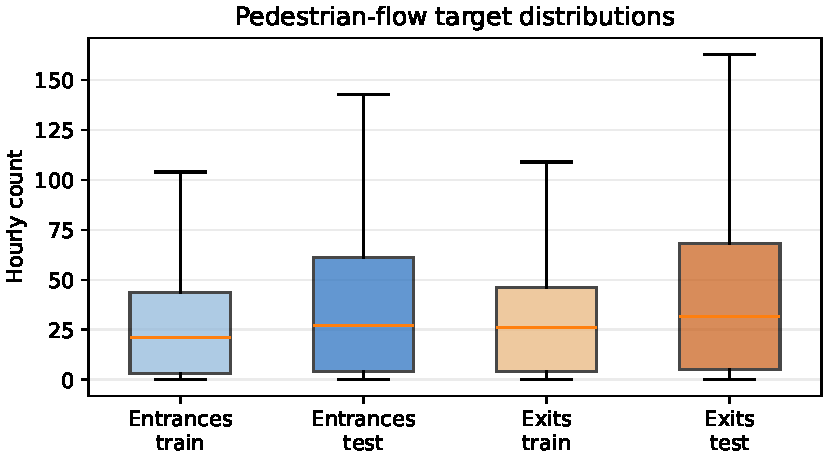
\includegraphics[width=0.86\textwidth]{flow_target_distribution_paper.pdf}
\caption{Pedestrian-flow target distributions in the chronological train and test splits. Outliers are hidden in the boxplot to keep the central range readable.}
\label{fig:flow-target-distribution}
\end{figure}

The pedestrian-flow targets are defined from the camera streams. The entrance
target ingressi\_borgo is the sum of entrances recorded by the Arcoribellino and
Piazzarocca Ingresso cameras. The exit target uscite\_borgo is the sum of exits
recorded by the Arcoribellino and Piazzarocca Uscita cameras. A timestamp is
marked complete only when the cameras needed for the target are present in the
same hour.

The TIM target families are derived from hourly mean-over-15-minute statistics.
The nationality track models Italian and foreign presences, while the age track
models six age-band presence indicators. The operational interpretation of the
TIM variables is shown in Table~\ref{tab:tim-dictionary}. The meanings are based
on the project data constraints and on public TIM City Forecast material
describing aggregated and anonymized mobile-network analytics for presence and
mobility monitoring \cite{TIMCityForecast,TIMAssisi}.

\begin{table}
\caption{Operational interpretation of the TIM fields used to derive presence, nationality, age, and mobility indicators.}
\label{tab:tim-dictionary}
\centering
\scriptsize
\begin{tabularx}{\textwidth}{lX}
\toprule
Fields & Meaning in this study \\
\midrule
event\_time; spatial fields & 15-minute timestamp and spatial identifiers for region, province, municipality, ACE area, and grid tile. \\
P, Ni, Ns & Total presences, Italian presences, and foreign presences; Ni + Ns = P in the raw data. \\
Tc, Tb & Italian consumer users with demographic detail and Italian business/non-consumer users; their sum approximates Ni. \\
Gm, Gf & Male and female aggregates within Tc; small differences may reflect rounding or unknown categories. \\
F1--F6 & Age bands within Tc: $<18$, 18--30, 31--40, 41--50, 51--60, and 61+. \\
Vp, Vr, Vi, Ve & Italian mobility categories: commuters, residents, intraregional visitors, and extraregional visitors. \\
mean15, sum15, max15 & Hourly mean, sum, and maximum over the 15-minute observations; sum15 is a person-quarter-hour aggregate. \\
\bottomrule
\end{tabularx}
\end{table}

\subsection{Preprocessing}

The preprocessing pipeline operates at hourly resolution. Pedestrian rows are
timestamped, grouped by hour, and aggregated into camera-level counts and
targets for the borough. TIM rows are converted from UTC to the Europe/Rome
analysis timezone, aggregated across tiles at 15-minute resolution, and then
summarized by hour using mean, sum, and maximum statistics. Weather measurements
from the local ERG5 grid are joined by hourly timestamp. Event records
are normalized into hourly active-count, intensity, scale, distance-band,
city-level, category-level, lagged, and rolling features. The final modeling
dataset is an inner join between complete pedestrian targets and TIM hourly
features, with weather and event covariates aligned on the same hourly
timestamp.

The inner join intentionally sacrifices the full pedestrian time span in order to
retain only hours where the main sources overlap. The pedestrian archive spans
from March 2022 to September 2025, while the joined modeling window is
restricted by TIM availability in 2025. The resulting testable dataset contains
2,735 hourly rows and 175 columns. This design is appropriate for cross-source
forecasting, but conclusions are limited to the observed TIM-overlap period.

\subsection{Forecasting setup and feature selection}

Experiments are run in forecast mode at 1, 3, 6, 12, and 24 hour horizons. The
main detailed tables report the one-hour horizon, while the multi-horizon
summaries and figures are used to assess robustness. The final evaluation uses a
chronological split with 2,164 training rows and 541 test rows. The train period
runs from 2025-03-04 18:00:00 to 2025-09-05 07:00:00; the test period runs from
2025-09-05 08:00:00 to 2025-09-30 22:00:00. Rolling validation summaries over
three folds are computed for every track and horizon.

\begin{table}
\caption{Experimental configuration used for the multi-horizon forecasting runs.}
\label{tab:setup}
\centering
\begin{tabularx}{\textwidth}{lX}
\toprule
Item & Value \\
\midrule
Forecast mode & forecast \\
Prediction horizons & 1, 3, 6, 12, and 24 hours \\
Primary reported horizon & 1 hour, with multi-horizon robustness tables \\
Train split & 2,164 rows, 2025-03-04 18:00:00 to 2025-09-05 07:00:00 \\
Test split & 541 rows, 2025-09-05 08:00:00 to 2025-09-30 22:00:00 \\
Lags & 1, 2, 24, and 168 hours \\
Rolling windows & 3, 6, and 24 hours \\
Execution nodes & CPU jobs ran on cnode04.hpc.prv and cnode06.hpc.prv, both in the cnode0[3-6] class: 2 x AMD EPYC 9454 48-Core CPUs and 512 GB DDR5 RAM per node \\
Slurm resources & Model jobs requested 4 CPU threads; 16 GB RAM for flow/nationality jobs and 24 GB RAM for age jobs \\
Top-k feature selection & Rolling validation over $k \in \{15,25,30,40,60\}$ for every track and horizon \\
Models & Persistence baselines, Ridge/log-Ridge, Poisson, Tweedie, Random Forest, Extra Trees, HGB, XGBoost, LightGBM, and two-stage Ridge \\
Interpretability & Permutation importance, SHAP, leave-one-group-out ablation, leave-one-feature-out ablation, and event-feature ablation summaries \\
\bottomrule
\end{tabularx}
\end{table}

Feature selection is leakage-aware. In forecast mode, same-hour variables from
the target family are excluded when they would reveal the future target, while
lagged and rolling historical variables are allowed. At the one-hour horizon,
the flow and nationality tasks start from 1,237 candidate features after leakage
exclusion and retain 265 and 264 features, respectively, after missingness and
collinearity filtering. The age task starts from 1,225 candidates and retains
264. The final top-k value is selected by rolling validation for every track and
horizon: at one hour, the selected values are 25 for flow and 15 for both
nationality and age.

The leakage rule is stricter than direct target removal. In forecast mode, all
unlagged TIM and pedestrian variables are excluded from feature models, because
they correspond to same-hour information at the forecast target time. Only
lagged and rolling versions of TIM and pedestrian variables are eligible. This
also prevents same-hour algebraic relationships among TIM fields, such as total
presence, nationality fields, consumer/business fields, and age-band fields,
from revealing the target. Calendar, weather, and event variables at the
forecast origin are retained, and quality or completeness flags are always
removed.

\begin{table}
\caption{Rolling-validation top-k selection by horizon and target family.}
\label{tab:top-k}
\centering
\scriptsize
\begin{tabular}{rlrrrr}
\toprule
Horizon & Track & Selected $k$ & Targets & Mean validation MAE & Mean validation $R^2$ \\
\midrule
1 h & flow & 25 & 2 & 16.65 & 0.672 \\
1 h & nationality & 15 & 2 & 56.36 & 0.876 \\
1 h & age & 15 & 6 & 20.72 & 0.802 \\
3 h & flow & 15 & 2 & 17.55 & 0.657 \\
3 h & nationality & 15 & 2 & 56.85 & 0.872 \\
3 h & age & 15 & 6 & 20.89 & 0.798 \\
6 h & flow & 15 & 2 & 17.64 & 0.645 \\
6 h & nationality & 15 & 2 & 56.42 & 0.874 \\
6 h & age & 15 & 6 & 20.77 & 0.801 \\
12 h & flow & 15 & 2 & 17.54 & 0.650 \\
12 h & nationality & 15 & 2 & 57.07 & 0.876 \\
12 h & age & 15 & 6 & 20.92 & 0.801 \\
24 h & flow & 15 & 2 & 17.44 & 0.656 \\
24 h & nationality & 15 & 2 & 56.42 & 0.882 \\
24 h & age & 15 & 6 & 20.76 & 0.807 \\
\bottomrule
\end{tabular}
\end{table}

\subsection{Models, metrics, and interpretation}

The model roster contains simple baselines and feature-based learners. Baselines
include mean and median dummy predictors, last-hour persistence, same-hour
previous-day/week predictors, and 24/168-hour rolling-mean predictors.
Feature-based models include ridge, log-ridge, Poisson, Tweedie, Random Forest,
Extra Trees, histogram gradient boosting, XGBoost, LightGBM, and a two-stage
ridge model. The tree-ensemble methods follow standard tabular-learning practice
\cite{Geurts2006ExtraTrees,Chen2016XGBoost,Ke2017LightGBM}.

Models are evaluated using MAE, RMSE, $R^2$, SMAPE, WAPE, MASE, peak-hour
classification metrics, training time, and inference time per row. WAPE is
emphasized when comparing targets with different scales, while MASE provides a
scale-normalized comparison against naive dynamics. Interpretation uses
selected-feature group counts, leave-one-group-out ablation,
leave-one-feature-out ablation, permutation importance, SHAP summaries, and
specific summaries for event-feature selection and event-feature ablation.
These artifacts are used as diagnostics of predictive dependence, not as causal
estimates. Leave-one-group-out ablation re-trains the selected feature model
after removing an entire feature family. Leave-one-feature-out ablation is more
local: for each target it re-trains the lowest-MAE feature-based model after
removing one selected feature at a time, without re-running hyperparameter
search.
Timing values are wall-clock
measurements collected with the same Python timing calls inside the CPU Slurm
jobs described in Table~\ref{tab:setup}; they support internal model comparison
within this pipeline rather than hardware-independent benchmarking.

\section{Results}
\label{sec:results}

All results in this section refer to the final chronological test split. Model
rankings are stated with the metric used for the ranking. Positive MAE gain
means that the feature-based model has lower MAE than the last-hour baseline;
positive ablation $\Delta$MAE means that removing the feature or feature family
increases MAE.

The pedestrian-flow task is the only target family for which feature-based
models lower one-hour MAE and WAPE relative to immediate persistence for both
targets. Table~\ref{tab:flow-results} reports the tree and boosting alternatives
with the lowest one-hour MAE, together with last-hour persistence.

\begin{table}
\caption{One-hour pedestrian-flow model leaderboard ranked by MAE on the final chronological test split.}
\label{tab:flow-results}
\centering
\scriptsize
\setlength{\tabcolsep}{3.5pt}
\begin{tabular}{llrrrrr}
\toprule
Target & Model & MAE & $R^2$ & WAPE & Fit s & ms/row \\
\midrule
ingressi\_borgo & Extra Trees & 18.69 & 0.554 & 37.81 & 0.50 & 0.119 \\
ingressi\_borgo & Random Forest & 19.23 & 0.545 & 38.90 & 0.68 & 0.080 \\
ingressi\_borgo & XGBoost & 19.89 & 0.539 & 40.24 & 0.31 & 0.005 \\
ingressi\_borgo & LightGBM & 20.98 & 0.524 & 42.42 & 0.17 & 0.006 \\
ingressi\_borgo & HGB & 21.16 & 0.508 & 42.80 & 0.43 & 0.014 \\
ingressi\_borgo & Last-hour & 21.29 & 0.636 & 43.06 & 0.00 & 0.010 \\
uscite\_borgo & Extra Trees & 15.39 & 0.826 & 28.93 & 0.50 & 0.099 \\
uscite\_borgo & Random Forest & 15.54 & 0.828 & 29.20 & 0.61 & 0.100 \\
uscite\_borgo & XGBoost & 15.66 & 0.821 & 29.42 & 0.31 & 0.005 \\
uscite\_borgo & HGB & 16.07 & 0.823 & 30.19 & 0.33 & 0.014 \\
uscite\_borgo & LightGBM & 16.22 & 0.807 & 30.49 & 0.17 & 0.006 \\
uscite\_borgo & Last-hour & 20.54 & 0.719 & 38.61 & 0.00 & 0.006 \\
\bottomrule
\end{tabular}
\end{table}

For entrances, Extra Trees reduces MAE by 12.2\% and WAPE by 5.3 percentage
points relative to last-hour persistence. For exits, it reduces MAE by 25.1\%
and WAPE by 9.7 percentage points. The $R^2$ ordering is different: last-hour
persistence has the highest $R^2$ for entrances, and Random Forest has the
highest $R^2$ for exits. The supported claim is therefore lower absolute error
for the Extra Trees flow forecasts, not universal dominance on every metric.
The close MAE values for Extra Trees, Random Forest, and XGBoost show that the
one-hour flow result is not tied to a single tree implementation.

The selected one-hour feature sets also differ by target family
(Table~\ref{tab:feature-groups}). Flow uses mostly recent camera-history
features, plus weather, calendar, TIM, and one target-history feature.
Nationality uses TIM, event, weather, and target-history features. Age uses TIM,
target-history, and one weather feature. Event variables are not selected for
one-hour flow or one-hour age models.

\begin{table}
\caption{One-hour selected-feature group composition, reported as counts of selected predictors by feature family.}
\label{tab:feature-groups}
\centering
\scriptsize
\begin{tabular}{lrrrrrrr}
\toprule
Track & Calendar & Events & Weather & Pedestrian & Target hist. & TIM & Total \\
\midrule
Flow & 2 & 0 & 6 & 14 & 1 & 2 & 25 \\
Nationality & 0 & 3 & 2 & 0 & 3 & 7 & 15 \\
Age & 0 & 0 & 1 & 0 & 8 & 6 & 15 \\
\bottomrule
\end{tabular}
\end{table}

The multi-horizon comparison in Table~\ref{tab:flow-horizon} limits the flow
claim to short horizons. Feature-based models improve over last-hour
persistence for both flow targets at one hour. At three hours only entrances
show a positive MAE gain. At six hours entrances improve by 8.4\%, while exits
are effectively tied with persistence (+0.2\% MAE gain). At 12 and 24 hours,
last-hour persistence has lower MAE than the best feature-based model.

\begin{table}
\caption{Pedestrian-flow comparison between last-hour persistence and the lowest-MAE feature-based model across horizons. Positive gain means lower MAE than persistence.}
\label{tab:flow-horizon}
\centering
\scriptsize
\begin{tabularx}{\textwidth}{rlXrrrr}
\toprule
Horizon & Target & Feature model & Last-hour MAE & Feature MAE & Feature $R^2$ & MAE gain \\
\midrule
1 h & ingressi\_borgo & Extra Trees & 21.29 & 18.69 & 0.554 & +12.20\% \\
1 h & uscite\_borgo & Extra Trees & 20.54 & 15.39 & 0.826 & +25.07\% \\
3 h & ingressi\_borgo & Random Forest & 21.39 & 21.13 & 0.438 & +1.22\% \\
3 h & uscite\_borgo & Random Forest & 20.63 & 20.96 & 0.611 & -1.62\% \\
6 h & ingressi\_borgo & Extra Trees & 21.56 & 19.76 & 0.558 & +8.37\% \\
6 h & uscite\_borgo & Extra Trees & 20.78 & 20.73 & 0.611 & +0.21\% \\
12 h & ingressi\_borgo & Extra Trees & 21.44 & 24.15 & 0.441 & -12.64\% \\
12 h & uscite\_borgo & Extra Trees & 20.75 & 26.87 & 0.443 & -29.51\% \\
24 h & ingressi\_borgo & XGBoost & 21.73 & 22.59 & 0.471 & -3.98\% \\
24 h & uscite\_borgo & XGBoost & 20.84 & 23.81 & 0.526 & -14.23\% \\
\bottomrule
\end{tabularx}
\end{table}

Figure~\ref{fig:flow-horizon-gain} visualizes the same comparison as a signed
MAE reduction relative to last-hour persistence. The figure is retained because
it makes the non-monotonic horizon behavior visible: the feature-based advantage
is largest at one hour, partly reappears for entrances at six hours, and is
negative at longer horizons.

\begin{figure}
\centering
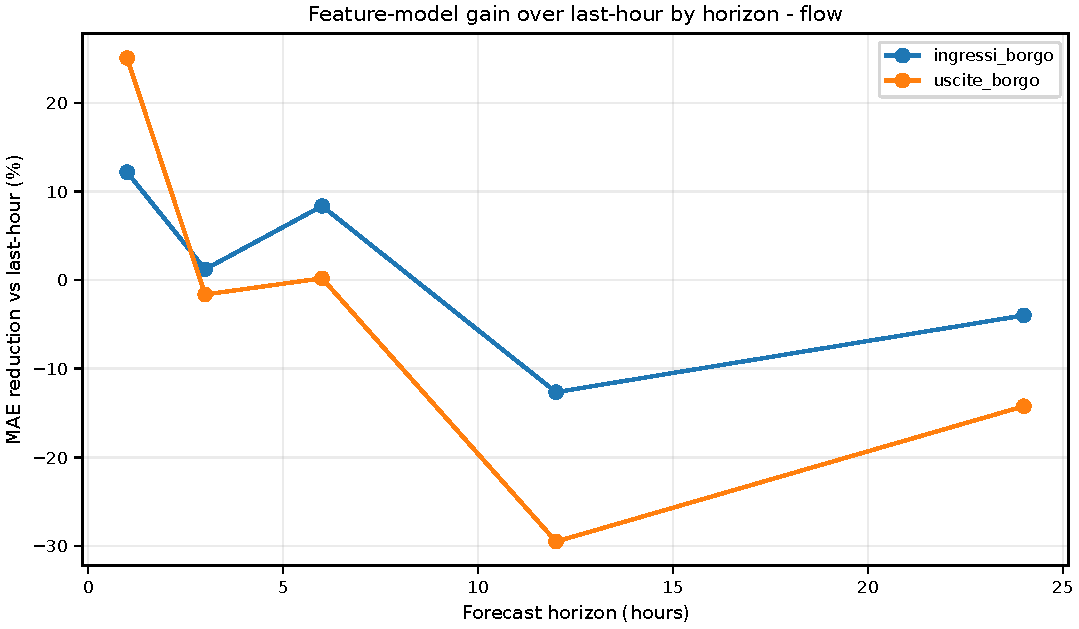
\includegraphics[width=0.78\textwidth]{feature_gain_vs_last_hour_by_horizon_flow.pdf}
\caption{Pedestrian-flow MAE reduction of the lowest-MAE feature model relative to last-hour persistence. Positive values mean lower MAE than persistence.}
\label{fig:flow-horizon-gain}
\end{figure}

Rolling validation gives a stricter temporal robustness check than the final
split alone. Table~\ref{tab:rolling-validation} reports the lowest-MAE model
averaged over three rolling folds at the one-hour horizon. For exits, Extra
Trees is also the rolling-validation winner. For entrances, rolling validation
selects last-hour persistence even though Extra Trees has lower MAE on the
final September test split. The entrance result is therefore a final-period
error reduction, while the exit result is supported by both rolling validation
and the final split.

\begin{table}
\caption{One-hour rolling-validation winners by target. Values are means over three chronological folds.}
\label{tab:rolling-validation}
\centering
\scriptsize
\setlength{\tabcolsep}{3.5pt}
\begin{tabular}{lllrrrr}
\toprule
Track & Target & Rolling winner & Folds & MAE mean & MAE std & $R^2$ mean \\
\midrule
Flow & entrances & Last-hour & 3 & 17.35 & 2.81 & 0.631 \\
Flow & exits & Extra Trees & 3 & 15.95 & 3.31 & 0.713 \\
Nationality & Italian & Last-hour & 3 & 102.38 & 26.85 & 0.886 \\
Nationality & foreign & Last-hour & 3 & 10.34 & 3.40 & 0.866 \\
Age & $<18$ & Last-hour & 3 & 5.15 & 0.97 & 0.711 \\
Age & 18--30 & Last-hour & 3 & 18.22 & 5.50 & 0.802 \\
Age & 31--40 & Last-hour & 3 & 18.49 & 4.41 & 0.833 \\
Age & 41--50 & Last-hour & 3 & 24.74 & 6.75 & 0.819 \\
Age & 51--60 & Last-hour & 3 & 29.07 & 5.60 & 0.841 \\
Age & 61+ & Last-hour & 3 & 28.64 & 4.57 & 0.809 \\
\bottomrule
\end{tabular}
\end{table}

TIM nationality and age targets have a different behavior. Table~\ref{tab:persistence}
shows that, at one hour, last-hour persistence has lower MAE than the
lowest-MAE feature-based model for all eight TIM targets. The same pattern holds across
all 40 TIM target-horizon cases in the complete multi-horizon target summary.
Feature-rich models often achieve
positive $R^2$, but their absolute error is higher than immediate persistence.
For these TIM indicators, the predictable component in this experiment is
therefore dominated by autoregressive continuity.

\begin{table}
\caption{Persistence versus the lowest-MAE feature-based model at the one-hour horizon for TIM targets.}
\label{tab:persistence}
\centering
\scriptsize
\begin{tabularx}{\textwidth}{llrrXrr}
\toprule
Track & Target & Last-hour MAE & Last-hour $R^2$ & Best feature model & Feature MAE & Feature $R^2$ \\
\midrule
Nationality & tim\_Ni\_mean15 & 97.80 & 0.858 & ridge & 157.88 & 0.604 \\
Nationality & tim\_Ns\_mean15 & 8.00 & 0.815 & Extra Trees & 12.00 & 0.626 \\
Age & tim\_F1\_mean15 & 4.91 & 0.711 & two-stage ridge & 10.13 & 0.191 \\
Age & tim\_F2\_mean15 & 15.26 & 0.787 & ridge & 21.14 & 0.457 \\
Age & tim\_F3\_mean15 & 16.60 & 0.800 & ridge & 25.02 & 0.488 \\
Age & tim\_F4\_mean15 & 21.88 & 0.792 & two-stage ridge & 34.45 & 0.446 \\
Age & tim\_F5\_mean15 & 27.47 & 0.848 & Extra Trees & 46.15 & 0.590 \\
Age & tim\_F6\_mean15 & 26.23 & 0.732 & HGB & 37.20 & 0.506 \\
\bottomrule
\end{tabularx}
\end{table}

Group-level ablation gives a coarse interpretation of the best feature-based
models. Table~\ref{tab:ablation} reports the feature family whose removal gives
the largest average one-hour MAE increase within each track. For flow, the
dominant family is pedestrian history. For nationality and age, the dominant
families are TIM-derived variables and target history. Weather and event
features can be selected, but their one-hour group-level effect is smaller than
the dominant history or TIM groups.

\begin{table}
\caption{Largest average MAE degradation under one-hour leave-one-group-out ablation. Positive values mean worse performance after removing the feature family.}
\label{tab:ablation}
\centering
\begin{tabular}{lcr}
\toprule
Track & Highest-impact removed group & Mean $\Delta$MAE \\
\midrule
Flow & pedestrian history & +6.01 \\
Nationality & TIM & +67.41 \\
Age & TIM & +9.20 \\
\bottomrule
\end{tabular}
\end{table}

The leave-one-feature-out ablation in Table~\ref{tab:single-feature-ablation}
is narrower than group ablation: it removes one selected feature at a time and
re-trains the lowest-MAE feature-based model for the affected target, without
retuning. It identifies local dependencies inside the selected feature set. For
one-hour flow, the largest single-feature effects are small in count units
relative to the group-level pedestrian-history effect. For TIM targets, the
largest single-feature effects are usually TIM or target-history lags, which is
consistent with the persistence-dominated performance comparison.

\begin{table}
\caption{Largest leave-one-feature-out MAE degradation by track and horizon, after re-training the selected feature-based model without one predictor.}
\label{tab:single-feature-ablation}
\centering
\scriptsize
\setlength{\tabcolsep}{2.5pt}
\begin{tabularx}{\textwidth}{rl l l X l r}
\toprule
Horizon & Track & Target & Model & Removed feature & Group & $\Delta$MAE \\
\midrule
1 h & Flow & \path|ingressi_borgo| & Extra Trees & \path|hour| & calendar & +0.85 \\
1 h & Nationality & \path|tim_Ni_mean15| & Ridge & \path|tim_Tc_mean15_lag1h| & TIM & +38.56 \\
1 h & Age & \path|tim_F6_mean15| & HGB & \path|tim_F6_mean15_lag1h| & target hist. & +12.96 \\
3 h & Flow & \path|uscite_borgo| & Random Forest & \path|entra_piazzarocca_ingresso_lag1h| & pedestrian & +0.65 \\
3 h & Nationality & \path|tim_Ni_mean15| & Extra Trees & \path|tim_Ns_mean15_lag1h| & target hist. & +19.29 \\
3 h & Age & \path|tim_F6_mean15| & Poisson & \path|tim_F6_sum15_roll24h_mean| & target hist. & +20.48 \\
6 h & Flow & \path|uscite_borgo| & Extra Trees & \path|tim_Vp_max15_roll6h_mean| & TIM & +1.88 \\
6 h & Nationality & \path|tim_Ni_mean15| & Ridge & \path|tim_F6_mean15_lag24h| & TIM & +21.53 \\
6 h & Age & \path|tim_F6_mean15| & Poisson & \path|tim_F6_sum15_roll24h_mean| & target hist. & +49.14 \\
12 h & Flow & \path|uscite_borgo| & Extra Trees & \path|tim_Vi_mean15_lag24h| & TIM & +0.95 \\
12 h & Nationality & \path|tim_Ni_mean15| & Poisson & \path|tim_Gf_mean15_roll24h_mean| & TIM & +238.03 \\
12 h & Age & \path|tim_F6_mean15| & HGB & \path|tim_F6_sum15_roll24h_mean| & target hist. & +104.55 \\
24 h & Flow & \path|uscite_borgo| & XGBoost & \path|tim_Vp_mean15_lag24h| & TIM & +4.95 \\
24 h & Nationality & \path|tim_Ni_mean15| & XGBoost & \path|tim_Gf_mean15_lag24h| & TIM & +16.66 \\
24 h & Age & \path|tim_F6_mean15| & XGBoost & \path|tim_F6_mean15_lag24h| & target hist. & +13.28 \\
\bottomrule
\end{tabularx}
\end{table}

The event-feature analysis is mixed. The event-aware dataset contains 42 event
features, and at least one event signal is non-zero in 2,132 of 2,735 modeling
hours. Table~\ref{tab:events} shows that event variables enter the selected
feature set mainly for nationality and age at 3--12 hours; they enter the flow
feature set only at six hours. The leave-one-group-out event effect is positive
for nationality at one, three, and six hours and for flow at six hours, but it
is negative for nationality at 12 and 24 hours and for age at 3, 6, and 12
hours. This is evidence of predictive association in some fitted models, not a
stable performance gain.

\begin{table}
\caption{Event-feature selection and leave-one-group-out event ablation by horizon and track. Positive $\Delta$MAE means removing event features worsens the selected feature-based model.}
\label{tab:events}
\centering
\scriptsize
\begin{tabular}{rlrrr}
\toprule
Horizon & Track & Event features & Event share & Mean event $\Delta$MAE \\
\midrule
1 h & flow & 0/25 & 0.0\% & -- \\
1 h & nationality & 3/15 & 20.0\% & +3.39 \\
1 h & age & 0/15 & 0.0\% & -- \\
3 h & flow & 0/15 & 0.0\% & -- \\
3 h & nationality & 3/15 & 20.0\% & +2.53 \\
3 h & age & 4/15 & 26.7\% & -0.04 \\
6 h & flow & 3/15 & 20.0\% & +0.64 \\
6 h & nationality & 5/15 & 33.3\% & +0.60 \\
6 h & age & 7/15 & 46.7\% & -0.92 \\
12 h & flow & 0/15 & 0.0\% & -- \\
12 h & nationality & 6/15 & 40.0\% & -20.13 \\
12 h & age & 8/15 & 53.3\% & -4.61 \\
24 h & flow & 0/15 & 0.0\% & -- \\
24 h & nationality & 2/15 & 13.3\% & -0.20 \\
24 h & age & 0/15 & 0.0\% & -- \\
\bottomrule
\end{tabular}
\end{table}

SHAP summaries support the same cautious interpretation. Some event variables
rank highly for individual targets: sport/motor event intensity is the top SHAP
feature for \path|tim_Ni_mean15| at three hours, for \path|tim_F5_mean15| and
\path|tim_F6_mean15| at six hours, and for \path|tim_F2_mean15| and
\path|tim_F5_mean15| at 12 hours. Those target-level rankings do not overturn
the ablation result: the event signal is visible in parts of the demographic
models, but the current event encoding does not produce a consistent reduction
in test error across tracks and horizons.

The main operational result is therefore narrow and explicit. For short-horizon
pedestrian-flow forecasting, recent camera dynamics plus selected contextual
covariates provide lower MAE and WAPE than immediate persistence at one hour.
For TIM nationality and age indicators, immediate persistence remains the
lowest-MAE forecasting baseline in this dataset. Event variables should be kept
as exploratory covariates and diagnostics, not presented as a validated driver
of forecast accuracy.

\section{Conclusions}
\label{sec:conclusions}

\red{This paper presented an AI-driven multi-source urban analytics framework
for people forecasting in the historic borough of Dozza. The framework combines
pedestrian camera counts, mobile-network indicators, weather observations, and
event-related information in a single hourly modeling pipeline. The updated
evaluation uses causal temporal baselines and an embargo between train and test,
so that the reported forecast errors do not rely on future target information.}

\red{The strongest empirical result concerns pedestrian-flow forecasting.
Feature-based tabular models, especially Extra Trees, consistently outperform
the strict last-hour baseline for entrances and exits across the evaluated
horizons. This indicates that recent pedestrian dynamics and contextual
variables provide useful information for visitor-flow prediction in a small
historic destination.}

\red{The TIM-derived targets show a more nuanced pattern. On the final
chronological test split, feature-based models often improve over last-hour
persistence for nationality and age-band targets. However, one-hour rolling
validation still selects last-hour persistence for those TIM targets. The
appropriate conclusion is therefore not that complex models always dominate,
but that their advantage depends on the target, horizon, and validation
protocol.}

\red{The interpretability analyses support this view. Pedestrian-history
features are most important for pedestrian-flow models. TIM and target-history
features dominate the demographic models. Event variables are selected and can
rank highly in SHAP summaries for some targets, but their ablation effect is
mixed. They should be treated as exploratory signals rather than as stable
drivers of forecast accuracy.}

\red{The study has three main limitations. First, the analysis is limited to
the period where all data sources overlap. Second, it studies one borough, so
external validity must be tested on other small tourism destinations. Third,
the event dataset is still incomplete and does not provide reliable measures of
attendance, media impact, or visitor attractiveness. Future work should extend
the observation period, improve the event representation, and replicate the
framework in other historic towns before operational deployment in real-time
decision-support systems.}

\clearpage
{\scriptsize
\setlength{\tabcolsep}{3pt}
\begin{longtable}{rllp{0.25\textwidth}rrrr}
\caption{Lowest-MAE final-split model for each target and forecast horizon.}\\
\toprule
H & Track & Target & Model & MAE & $R^2$ & WAPE & MASE \\
\midrule
\endfirsthead
\toprule
H & Track & Target & Model & MAE & $R^2$ & WAPE & MASE \\
\midrule
\endhead
\midrule
\multicolumn{8}{r}{Continued on next page}\\
\endfoot
\bottomrule
\endlastfoot
1 h & age & \path|tim_F1_mean15| & \path|last_hour| & 4.91 & 0.711 & 7.12 & 0.43 \\
1 h & age & \path|tim_F2_mean15| & \path|last_hour| & 15.26 & 0.787 & 4.18 & 0.39 \\
1 h & age & \path|tim_F3_mean15| & \path|last_hour| & 16.60 & 0.800 & 3.72 & 0.39 \\
1 h & age & \path|tim_F4_mean15| & \path|last_hour| & 21.88 & 0.792 & 3.30 & 0.39 \\
1 h & age & \path|tim_F5_mean15| & \path|last_hour| & 27.47 & 0.848 & 3.13 & 0.42 \\
1 h & age & \path|tim_F6_mean15| & \path|last_hour| & 26.23 & 0.732 & 1.71 & 0.41 \\
1 h & flow & \path|ingressi_borgo| & \path|extra_trees| & 18.69 & 0.554 & 37.81 & 0.73 \\
1 h & flow & \path|uscite_borgo| & \path|extra_trees| & 15.39 & 0.826 & 28.93 & 0.54 \\
1 h & nationality & \path|tim_Ni_mean15| & \path|last_hour| & 97.80 & 0.858 & 2.06 & 0.39 \\
1 h & nationality & \path|tim_Ns_mean15| & \path|last_hour| & 8.00 & 0.815 & 6.73 & 0.23 \\
3 h & age & \path|tim_F1_mean15| & \path|last_hour| & 4.93 & 0.712 & 7.15 & 0.43 \\
3 h & age & \path|tim_F2_mean15| & \path|last_hour| & 15.28 & 0.789 & 4.18 & 0.38 \\
3 h & age & \path|tim_F3_mean15| & \path|last_hour| & 16.47 & 0.805 & 3.69 & 0.38 \\
3 h & age & \path|tim_F4_mean15| & \path|last_hour| & 21.84 & 0.795 & 3.30 & 0.38 \\
3 h & age & \path|tim_F5_mean15| & \path|last_hour| & 27.33 & 0.851 & 3.12 & 0.40 \\
3 h & age & \path|tim_F6_mean15| & \path|last_hour| & 26.30 & 0.737 & 1.72 & 0.40 \\
3 h & flow & \path|ingressi_borgo| & \path|random_forest| & 21.13 & 0.438 & 42.57 & 0.80 \\
3 h & flow & \path|uscite_borgo| & \path|last_hour| & 20.63 & 0.719 & 38.61 & 0.70 \\
3 h & nationality & \path|tim_Ni_mean15| & \path|last_hour| & 97.22 & 0.863 & 2.05 & 0.37 \\
3 h & nationality & \path|tim_Ns_mean15| & \path|last_hour| & 7.96 & 0.818 & 6.69 & 0.23 \\
6 h & age & \path|tim_F1_mean15| & \path|last_hour| & 4.93 & 0.715 & 7.15 & 0.43 \\
6 h & age & \path|tim_F2_mean15| & \path|last_hour| & 15.19 & 0.791 & 4.15 & 0.38 \\
6 h & age & \path|tim_F3_mean15| & \path|last_hour| & 16.34 & 0.810 & 3.65 & 0.38 \\
6 h & age & \path|tim_F4_mean15| & \path|last_hour| & 21.60 & 0.801 & 3.26 & 0.37 \\
6 h & age & \path|tim_F5_mean15| & \path|last_hour| & 26.87 & 0.857 & 3.06 & 0.39 \\
6 h & age & \path|tim_F6_mean15| & \path|last_hour| & 26.26 & 0.744 & 1.71 & 0.40 \\
6 h & flow & \path|ingressi_borgo| & \path|extra_trees| & 19.76 & 0.558 & 39.67 & 0.74 \\
6 h & flow & \path|uscite_borgo| & \path|extra_trees| & 20.73 & 0.611 & 38.65 & 0.70 \\
6 h & nationality & \path|tim_Ni_mean15| & \path|last_hour| & 95.67 & 0.871 & 2.02 & 0.37 \\
6 h & nationality & \path|tim_Ns_mean15| & \path|last_hour| & 7.99 & 0.814 & 6.70 & 0.23 \\
12 h & age & \path|tim_F1_mean15| & \path|last_hour| & 4.96 & 0.709 & 7.20 & 0.43 \\
12 h & age & \path|tim_F2_mean15| & \path|last_hour| & 15.27 & 0.790 & 4.17 & 0.38 \\
12 h & age & \path|tim_F3_mean15| & \path|last_hour| & 16.52 & 0.805 & 3.69 & 0.38 \\
12 h & age & \path|tim_F4_mean15| & \path|last_hour| & 21.72 & 0.798 & 3.27 & 0.37 \\
12 h & age & \path|tim_F5_mean15| & \path|last_hour| & 27.11 & 0.854 & 3.09 & 0.39 \\
12 h & age & \path|tim_F6_mean15| & \path|last_hour| & 26.46 & 0.715 & 1.72 & 0.40 \\
12 h & flow & \path|ingressi_borgo| & \path|last_hour| & 21.44 & 0.637 & 43.11 & 0.80 \\
12 h & flow & \path|uscite_borgo| & \path|last_hour| & 20.75 & 0.720 & 38.75 & 0.70 \\
12 h & nationality & \path|tim_Ni_mean15| & \path|last_hour| & 96.27 & 0.866 & 2.03 & 0.37 \\
12 h & nationality & \path|tim_Ns_mean15| & \path|last_hour| & 7.88 & 0.815 & 6.62 & 0.22 \\
24 h & age & \path|tim_F1_mean15| & \path|last_hour| & 5.00 & 0.702 & 7.29 & 0.45 \\
24 h & age & \path|tim_F2_mean15| & \path|last_hour| & 15.34 & 0.789 & 4.20 & 0.39 \\
24 h & age & \path|tim_F3_mean15| & \path|last_hour| & 16.70 & 0.805 & 3.74 & 0.39 \\
24 h & age & \path|tim_F4_mean15| & \path|last_hour| & 22.00 & 0.790 & 3.32 & 0.39 \\
24 h & age & \path|tim_F5_mean15| & \path|last_hour| & 27.43 & 0.848 & 3.13 & 0.41 \\
24 h & age & \path|tim_F6_mean15| & \path|last_hour| & 26.42 & 0.726 & 1.72 & 0.41 \\
24 h & flow & \path|ingressi_borgo| & \path|last_hour| & 21.73 & 0.635 & 43.07 & 0.83 \\
24 h & flow & \path|uscite_borgo| & \path|last_hour| & 20.84 & 0.719 & 38.44 & 0.73 \\
24 h & nationality & \path|tim_Ni_mean15| & \path|last_hour| & 97.32 & 0.857 & 2.05 & 0.38 \\
24 h & nationality & \path|tim_Ns_mean15| & \path|last_hour| & 7.87 & 0.823 & 6.62 & 0.22 \\
\end{longtable}
}


\subsection*{Acknowledgments}
\small
Research funded by the Industrial Research Project "Support System for Sustainable Smart Cities (S4C)" funded by the Emilia-Romagna PR FESR 2021–2027 under the Smart Specialisation Strategy (S3) and by the Development and Cohesion Fund, CUP E27G22000310007.
\bibliographystyle{splncs04}
\bibliography{references}

\end{document}
